\documentclass[twocolumn]{article}

\usepackage[utf8]{inputenc} %Para configuración de caracteres
\usepackage[spanish]{babel} %Para configuración de idioma
\usepackage{graphicx}
\usepackage{amsmath}
\usepackage{amsfonts}
\usepackage{float}
\let\olditemize\itemize
\def\itemize{\olditemize\itemsep=0pt } %%Reducir espacio itemize

\title{	
\includegraphics[scale=0.2]{univalle.jpg} \\ Taller 2 Estructuras de datos\\FUNDAMENTOS DE ANÁLISIS Y DISEÑO DE ALGORITMOS}
\author{Carlos Andres Delgado S, Ing \footnote{ carlos.andres.delgado@correounivalle.edu.co }}
\date{Mayo 2017}

\begin{document}
\maketitle

Este taller se puede trabajar en grupos de hasta 3 personas. Se debe entregar el código fuente de su solución y un breve informe en formato PDF que contenga:

\begin{itemize}
	\item Breve explicación de como soluciona el problema.
	\item Como se ingresan entradas a su algoritmo (lectura archivo, digitación entradas, etc).
	\item Que formato tiene la salida (impresión en pantalla, archivo).
	\item Presentación salida (Cómo se interpreta su salida, es decir como se puede entender).
	\item Ejemplo de ejecución de su algoritmo.
\end{itemize}

\textbf{Importante:} En este taller se propone \textbf{Java} como lenguaje de trabajo para la solución, pero usted es libre de usar cualquier otro lenguaje de su preferencia siempre y cuando maneje Objetos y Clases.

\section{Combinando listas ordenadas \\ \small{[25 puntos]}}

Desarrolle la operación \textbf{combinar(Lista L1, Lista L2)} que recibe dos listas simplemente
enlazadas, cada una ordenada ascendentemente, y devuelve una lista L3 que tiene los
elementos ordenados de ambas listas. Las listas pueden tener elementos repetidos. A
continuación se muestra un ejemplo.

\begin{figure}[H]
	\centering
	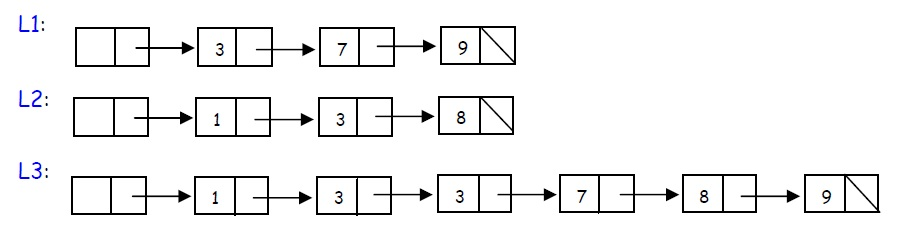
\includegraphics[scale=0.4]{ListaEnlazada.jpg}
	\caption{Ejemplo combinando lista enlazadas}
\end{figure}



\section{El inventario \small{[30 puntos]}}

En un museo se guarda la información del inventario de sus obras utilizando una lista
simplemente enlazadas en la que el campo dato es un objeto de la clase Obra. Una Obra en el
inventario tiene dos atributos \textbf{nombre y cantidad}.

\begin{itemize}
	\item Desarrolle la operación \textbf{agregarReplica(String nombre}), de tal forma que si no existe la obra con el nombre especificado, se crea en el inventario con cantidad 1. Si ya existe, se aumenta en 1 su cantidad. La lista debe estar ordenada de acuerdo el nombre.
	\item Desarrolle la operación \textbf{venderReplica(String nombre)}, de tal forma que si no hay obras disponibles con el nombre especificado se indique con un mensaje. En caso contrario, se disminuye en 1 su cantidad. Si una obra llega a la cantidad 0, se elimina el nodo de la lista.
	\item Desarrolle la operación \textbf{ListarReplicas()} que muestra para cada obra, su nombre y la cantidad disponible
\end{itemize}

Suponga que se tiene la siguiente lista:

\begin{figure}[H]
	\centering
	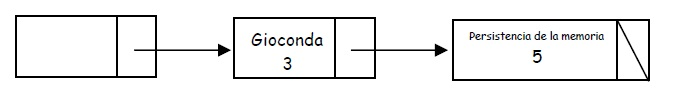
\includegraphics[scale=0.4]{ListaEnlazadaOp1.jpg}
	\caption{Lista enlazada de ejemplo}
\end{figure}

En la siguiente figura si se utiliza la operación \textbf{agregarReplica(``El hombre de Vitrubio'')}, la lista quedará de la siguiente manera:

\begin{figure}[H]
	\centering
	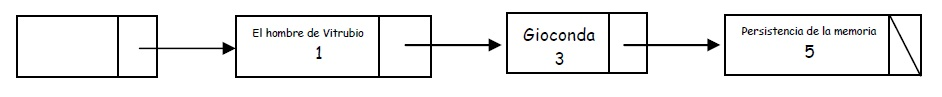
\includegraphics[scale=0.35]{ListaEnlazadaOp2.jpg}
	\caption{Lista enlazada con operación agregar réplica}
\end{figure}

Si después se utiliza la operación \textbf{venderReplica("Gioconda")}, la lista debe tener el siguiente estado:

\begin{figure}[H]
	\centering
	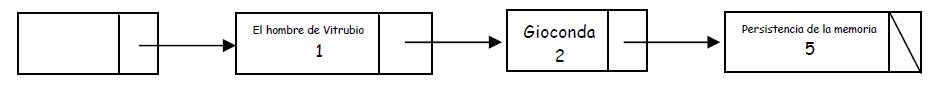
\includegraphics[scale=0.35]{ListaEnlazadaOp3.jpg}
	\caption{Lista enlazada con operación vender réplica}
\end{figure}

\section{Implementando una pila con colas \small{[20 puntos]}}

Utilizando la estructura Cola, desarrolle las siguientes operaciones básicas de una Pila:

\begin{itemize}
	\item public boolean \textbf{estaVaciaPilaConColas()}
	\item public void \textbf{pushPilaConColas(Object o)}
	\item public Object \textbf{popPilaConColas()}
	\item public void \textbf{mostrarPilaConColas()}
\end{itemize}

\section{Dominó modificado \small{[25 puntos]}}

Se requiere una aplicación para el juego dominó modificado, en donde sólo existen para cada posible par de números únicos desde el 1 hasta el 9 (Ejemplo: $1+2, 1+3, 1+4, 1+5, 1+6, 1+7, 1+8, 1+9, 2+3, 2+4, 2+5, . . . $). Note que no existen las piezas simétricas $1+2$ y $2+1$ en el conjunto, ya que cada una de estas piezas puede convertirse en la otra rotándola. Implemente una estructura de datos que permita:

\begin{itemize}
	\item Crear inicial el conjunto de 36 fichas de dominó. Cada ficha tiene dos estados, el primero que indica si se encuentra utilizada o disponible y el segundo su rotación hacia la derecha $(0º,90º,180º,270º)$. Se asumen que la forma mostrada en la figura \ref{fig:dominoSet} están a $0º$ de rotación, para ver las rotaciones de una ficha se puede consultar la figura \ref{fig:dominoRotacion}.
	\item Extraer una ficha, marcando esta como utilizada.
	\item Ingresar una ficha y en el caso que este marcada como utilizada, se marca como disponible.
	\item Un método para buscar una ficha a partir de sus valores $A$, $B$ e imprimir si esta está disponible o no y su rotación. Por ejemplo para buscar la ficha $1,2$ los valores son $A=1$, $B=2$. 
\end{itemize}

En la siguiente figura se muestra el conjunto de fichas disponibles:

\begin{figure}[H]
	\centering
	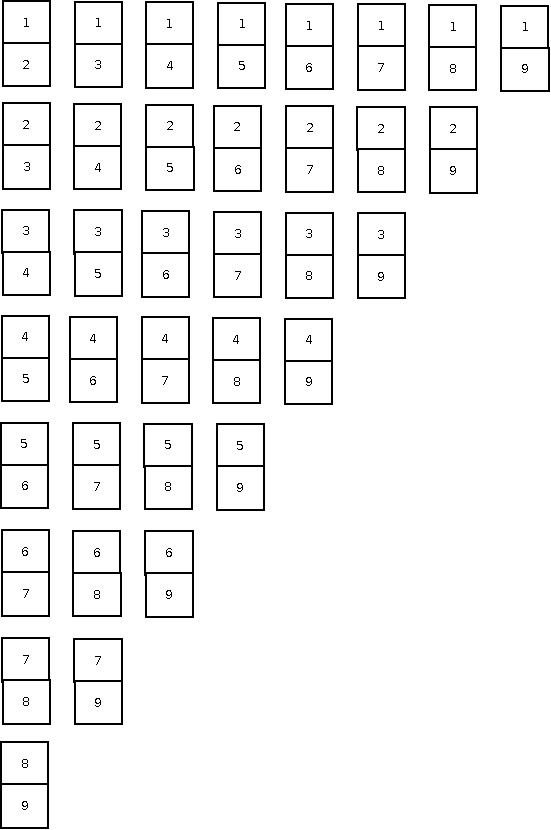
\includegraphics[scale=0.5]{domino-set.jpg}
	\caption{Fichas de dominó}
	\label{fig:dominoSet}
\end{figure}

La rotación de una ficha se puede ver de la siguiente manera:
\begin{figure}[H]
	\centering
	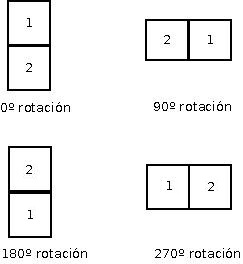
\includegraphics[scale=0.6]{Rotaciones.jpeg}
	\caption{Rotaciones de una ficha de dominó}
	\label{fig:dominoRotacion}
\end{figure}



Justifique en términos de operaciones: inserción y borrado porque su estructura de datos es apropiada para solucionar este problema.

\end{document}
